\section{Literature Review}
Creating lower frequency waves from higher frequency waves by non-linear interaction began in the field of sonar through development of underwater sonar techniques as far back as the 1960's in a publication by Westervelt \cite{westervelt_1963}. These developments produced a formal mathematical basis for the effect of directive ultrasonic transducers arrays and were referred to as parametric arrays.\\
While these sonar systems were developed for underwater use, a publication in 1975 by the Acoustical Society of America \cite{bennett_blackstock_1975} revealed that the nonlinear effects observed underwater could occur in air as well.\\
By 1983, companies such as Ricoh \cite{yoneyama_fujimoto_kawamo_sasabe_1983} developed directional loudspeaker systems; however, found them quite costly to consider as a viable product for exhibits and museum installations. Their implementations were rudimentary with basic equalisation of the audio signal and double side band amplitude modulation. They identified a proportional relationship between the modulation depth ($m)$ and the sound pressure of the signal; however, found that the distortion is proportional to $m^2$.\\
By 1998, Kite \cite{kite_post_hamilton_1998} proved that the distortion can be reduced by preprocessing this signal appropriately. Pompei \cite{pompei2002sound} implemented the square root amplitude modulation (SRAM) technique proposed by Kite which overcame the squaring of the envelope signal first identified by Berktay's approximation. This reduced the harmonic distortion compared to Double Side Band Amplitude Modulation (DSBAM) used before.\\
Kite \cite{kite_post_hamilton_1998} noted that the distortion can be totally removed if the harmonics of the modulating signal created by the square root process in SRAM are reproduced by the ultrasonic transducers themselves. However, this would require an infinite bandwidth in the ideal case or atleast more than 10 kHz of bandwidth for each transducer in the array which was found to be infeasible.\\
The past innovations in the field neglected to consider the bandwidth of the transducers themselves. In 2009, Tan et al. \cite{tan2010preprocessing} tackled this problem by considering a different modulation approach using Modified Amplitude Modulation (MAM). This modulation scheme involved a form of quadrature amplitude modulation which took into account the 3dB bandwidth of the transducers themselves. This further lowered the distortion present in the demodulated signal. By 2012, Gan et al. \cite{gan2012review} reviews the existing techniques in the directional audio phenomenon with a glimpse into new related works. During this review the theoretical framework of parametric acoustic arrays is discussed where primary and secondary beams are described as a result of fundamental and difference frequency components. The secondary source column of the difference frequency creates a virtual secondary beam within the primary beam as shown in the figure created by Gan et al. re-presented in figure \ref{fig:ganprisec}\cite{gan2012review}. A practical demonstration of the directionality phenomenon is shown through simulation and is reiterated in figure \ref{fig:gandirectionality}\cite{gan2012review} where a single element speaker is compared to a parametric speaker (with matching 10cm radius) producing an audible 2 kHz tone from its secondary beam using an ultrasonic 40 kHz primary beam.
\begin{figure}[ht!]
    \centering
    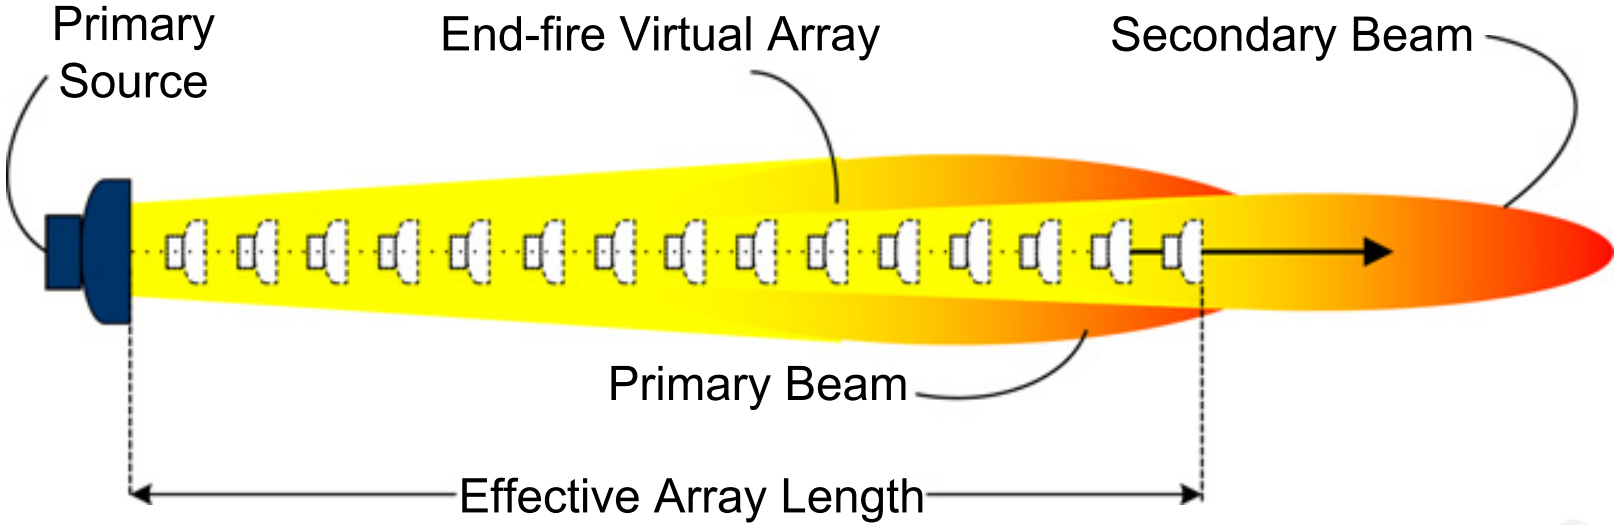
\includegraphics[width=0.65\textwidth]{Figures/primsecbeamarrayGan2012review.png}
    \caption{Functional diagram created by Gan et al. demonstrating primary and resulting secondary beams created from a parametric acoustic array.}
    \label{fig:ganprisec}
\end{figure}
\begin{figure}[ht!]
    \centering
    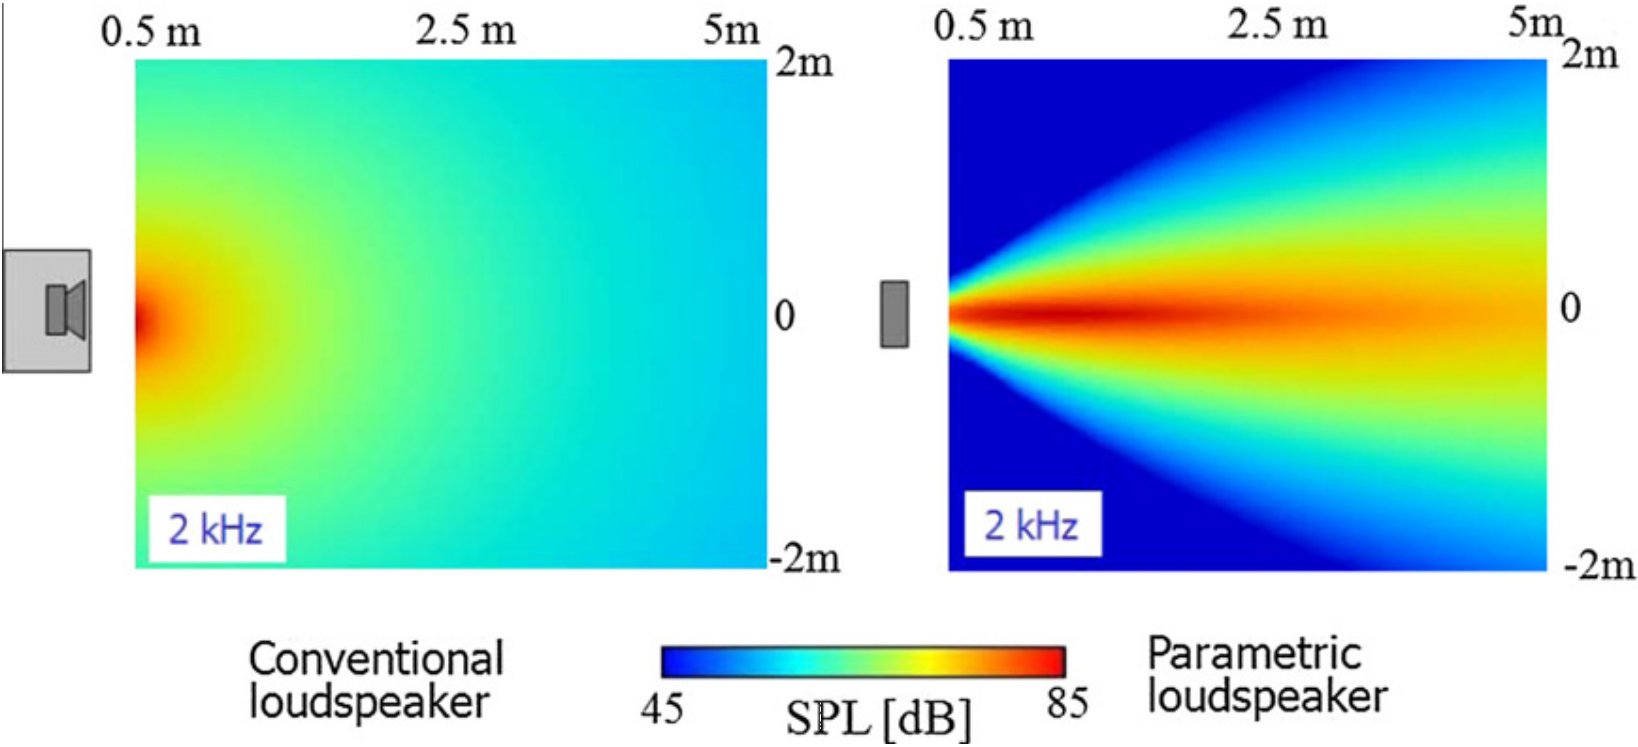
\includegraphics[width=0.5\textwidth]{Figures/2khzDirectionalitygan2012review.png}
    \caption{Simulated comparison between conventional and parametric loudspeakers created by Gan et al.}
    \label{fig:gandirectionality}
\end{figure}

Recent studies suggest that the harmonic distortion is related to the frequency response of the ultrasonic transducers not being considered in Berktay's equation; however, a paper from 2018 \cite{farias_abdulla_2018} suggests this can be overcome by choosing a suitable modulation technique and applying a filter which describes the transducer array's frequency response.\\
%Mentioning existing products
In terms of real world applications of directional audio systems, Dr. Pompei went on to further develop his directional Audio Spotlight at the MIT Media Lab during his Ph.D. and founded Holosonics to commercialise the technology. This resulted in the technology finding application in museums and galleries, digital signage, libraries, hospitals and retail settings \cite{holosonicsresearchlabs_2002}.
%what I'm going to do
In review of the major prior works done in the field of directional acoustics; progress towards a viable directional audio system is feasibile in both commercial and academic settings. While a lot of the techniques used by these prior works show great promise for a high quality directional audio system, they make little mention of the costs involved in producing such a system since their focus is on perfecting their individual techniques. Holosonic's products show commercial feasibility of this system but have price ranges of between \$500 to \$2000 and as a result are not low cost implementations. The directional audio system discussed in this report aims to produce a low cost implementation with the potential to be further iterated on to improve its quality in the future. This low cost implementation will likely be far more rudimentary than these systems given the previously mentioned scope and limitations of the project, thus cannot be directly compared to the outputs of the above mentioned works. Rather, the techniques used in these prior works will be implemented where possible and explored to identify a middle ground between a feasible, low cost implementation and a quality directional audio output device.